\newpage
\section{The Serval Networking Architecture}
\subsection{Introduction}
Serval\footnote{More information about the Serval Architecture can be found in the presentation in the Appendix (\ref{sec:servaldhtpres}).} is an end-host stack evolving into a service-centric network architecture, proposed and prototyped by the \href{https://sns.cs.princeton.edu/}{systems and networking group} at \href{https://www.princeton.edu}{Princeton University}, in 2012.

\paragraph{} In the original paper "A Service Access Layer, at Your Service" (2011)\cite{Freedman2011} and later on "Serval: An End-Host Stack for Service-Centric Networking" (2012)\cite{Nordstrom2012}, Freedman, Nordstr{\"o}m et. al. first decompose the needs of modern networked applications, locate the discordances with the current Network Stack, study previous work and how each of them individually fails to stand as a proper solution, rethink the current TCP/IP Networking Stack and propose two simple abstractions that can obliterate the legacy problems discussed on Problem Definition (\ref{problemdefinition}).\\
\indent Furthermore they investigate how those abstractions fit in a new 3.5 layer, the Service Access Layer (SAL)\nomenclature{SAL}{Service Access Layer}, and emphasize on the clean service-level data/control plane separation it imposes.
Additionally, they review a formally-verified end-to-end connection control protocol (ECCP) \nomenclature{ECCP}{End-to-End Connection Control Protocol} [TODO], which elevates services to first-class citizens.
After all, they focus on the SAL prototype and the lessons learned from building it.

\subsection{Proposed abstractions}
As will be discussed later on at the section "Review of Relative Bibliography" (\ref{sec:reviewbibliography}), various abstractions have been proposed in order to support the concept of Service-Centric networking.
Deciding the right abstractions premises first the detailed understanding of where a problem resides, and then the genuine intuition for conceiving the simple yet powerful generalizations that better conform with the current and future needs.
Those abstractions should be transparent enough for legacy ports and hot swapping with the prevalent systems, in the meantime powerful to break ground for future advancements.\\
\indent We appraise the Serval abstractions of \emph{Service Names} and \emph{Flow Identifiers} for being a great solution on the overloading of identifiers within and across the present TCP/IP stack.
Also, for the tight fit of those abstractions in the separation of data and control plane.
Finally, it is remarkable how the adoption of those abstractions requires minimal if no modifications at all in the infrastructure that powers networks today.

\subsubsection{Service Names}
The main idea behind Service-Centric Networking is that nowadays network users request services by their names and are completely agnostic of the underlying procedures.
Hereby an abstraction is needed for identifying a service, resolving and of course effectively routing a request to an instance of that service, according to specific rules.
For that reason Serval introduces service names, or \emph{serviceIDs}.\\
\indent ServiceIDs are large (256 bit long) strings, that correspond to a service, or a group of services.
Part of Serval packets as a Service Access Extension header in the synchronization process (SYN and SYN-ACK flags in ECCP state machine figure \ref{fig:ECCP_st}), serviceIDs assist in resolution and service-level routing.
Furthermore they are used as persistent, global identifiers for easier handling of replicated services, virtual machine migrations or mobile hosts, when there is a need for end-point signaling.\\
\indent What is unique about Serval's adifferencebstraction of service identifiers is that since they are managed by the SAL, they are positioned below the transport layer.
Jointly with Serval active sockets, the abstraction of service names obscures host identifiers (IP and Port) from the application layer, but stills offers powerful, familiar APIs\nomenclature{API}{Application Programming Interface} to networked application developers.
\indent service granularity (block allocation) \\
\indent To sum up, in an elegant way serviceIDs promote services to the principal entities in the network, by giving applications intermediate access to the service control plane and a
And it manages to do so while hiding unneeded abstractions, such as the $<IP, port>$ tuple.

\subsubsection{End-host flow identifiers}
The other problem Serval is intending to counteract, is the 

\subsection{Service Resolution}
Those service names in a deeper level get mapped to 
human readable strings similar to domain names, for identifying services.
regardless it's geographical position, the port it is bound, 

\subsubsection{Hierarchical Resolution}
Relative to today's domain name system, those serviceIDs can be mapped to human-readable strings, much like URIs.

\subsubsection{Flat Resolution Schemes}
Another approach suggests that serviceIDs are calculated by a hash function on a service prefix and an application-level instance unique key.
This practice of a \emph{semantic-free, flat} namespace better supports networks without a hierarchical structure, like datacenter and Wide Area networks.
By semantic-free\cite{Walfisha2004} reference we mean that by default 

\subsection{Service-Level Routing} 
No need for deep packet inspection in load balancers


\subsubsection{Late binding}

\subsection{Serval Network Stack}
Extra points go to Serval for being transport-protocol agnostic.
This means that developers may choose to use either TCP, UDP\nomenclature{UDP}{User Datagram Protocol}, ATP\nomenclature{ATP}{AppleTalk Transaction Protocol}, FCP\nomenclature{FCP}{Fibre Channel Protocol} or actually any transport protocol, since it is supported by SAL, without modifying the source code of their application.
This opens new windows for experimentation and innovation.

\subsubsection{Service Controller}

\subsubsection{Service Access Layer}
extremes
\subsubsection{Serval Packets Structure}

\subsection{Incremental migration to Serval}
With Serval being actively under development, it is time to discuss the deployment approaches that could guide us to something that has never happened before; the wide adoption of a new network stack.
Above all, benchmarks prove that introducing Serval in large scale networks as well as datacenters offers a wide range of new functionality in speeds comparable to the original TCP/IP stack ones. However, with Internet being a massive diverse network controlled distributively by assorted interest groups --vendors, ISPs, service providers--, deployment of a new networking architecture is a real nightmare \cite{Podmayersky2011}.
\\ \indent Prime example is the adoption of IPv6. Intending to solve the problem of IPv4 exhaustion, IPv6 uses 128-bit addresses (in comparison to IPv4's 32-bit IP addresses), providing approximately 4.3 billion addresses for network interfaces. Still, after over a decade of protracted efforts, less than 4\% \footnote{Visualization based on original data from RIR, routeviews, Alexa, Google, ITU and APnic by Cisco at \url{http://6lab.cisco.com/stats/}} of Internet global traffic is carried over it, although it is a necessary to take step for the next generation of the Internet of Things. \nomenclature{IoT}{Internet of Things}
\\ \indent A smooth transition to a new architecture requires two things: first that current hardware and intermediary devices are compatible or at least do not interfere with the new packet headers, and that applications are utilizing the late interfaces and are able to dissect and synthesize those packets.

\subsubsection{Legacy Hardware}
SAL's position just on top of the network layer makes it translucent to networking equipment such as hubs, switches and routers, since they are messing up with the headers of up to the network layer.
At this level, hardware is responsible only for delivering the packets to the right destination, the way they have been doing so far.
\\ \indent Serval on the contrary is not immune to stateful packet inspection\nomenclature{SPI}{Stateful Packet Inspection} and deep packet inspection\nomenclature{DPI}{Deep Packet Inspection}.
Intermediaries who access the headers of the transport or above layers will have a hard time dissecting a minimum 32 extra bytes following the network layer.
The use of NAT-based\nomenclature{NAT}{Network Address Translator} agents though, such as load balancers, can be obscured due to the late binding on serviceIDs.
In any way, operation behind legacy networks middleware can be achieved via UDP encapsulation.
\\ \indent Apparently, even if typical routers are compatible with routing Serval packets, they cannot provide service-level routing, service registration, unregistration and propagation, or any other feature of a Serval router\footnote{The generation of routers that supports virtual services, such as the Cisco Nexus series 1100, might be able to imitate features of a service router with a virtual service.}.
Hopefully this is not a blocking obstacle, as far as the SAL knows a service router that can forward service name resolution requests to.
That service router might be deep within the network and not accessible through service propagation.

\subsubsection{Modified Programming Interfaces}
Unlike other proposals which can be either integrated in programs as libraries or provide abstractions by overloading identifiers such as ports, Serval's kernel module implementation requires applications to be modified in order to use its active sockets API.
\\ \indent In other words, a minimum port of an existing applications would require to include and link to \textless libserval/serval.h\textgreater ~and \textless netinet/serval.h\textgreater ~libraries, set socket family to AF\_SERVAL and substitute system calls to the socket layer such as connect, bind, accept, send etc to use serviceIDs.
Minor modifications might be needed, since new identifiers require different size of bytes to be allocated in memory and so on.
\\ \indent The complexity of porting an existing application to Serval depends on how neatly is the connection module isolated.
In general, applications that support various protocols are easier to be ported, since connectivity functions are already decoupled from the program logic and can be replicated to support new APIs.
Large applications, with thousands lines of code,\nomenclature{loc}{lines of code} like Mozilla Firefox require modifications in around just 70 lines of code.
Design patterns like singleton and factory noticeably indicate which parts of the source code should be altered.
\\ \indent Nevertheless, applications can simultaneously support multiple protocols and stacks, according to the requests of the other end.
This will be a great advantage in the transitory period of large scale deployment.
\\ \indent On the other hand, unexpected runtime results might be confronted due to overlapping of features offered by SAL and reimplemented in the program.
For instance service load balancing at SAL, an inherent component of Serval, might muddle with the application-specific way of allotting requests.
In such cases if possible one of the methods should dominate the final decision.
Either a unique serviceID of an allocated serviceID block --as described in the Hierarchical Resolution approach-- should be used for each instance, and let load-balancing be made by application's functions.
Or load-balancing logic within the application should be removed when a socket's family is AF\_SERVAL and be managed according to service-level rules defined in SAL.
\\ \indent As a reference you can find a diff file from the port of nginx\footnote{Nginx [engine-ex] is an Open Source HTTP, reverse proxy and mail proxy server\\ \url{http://nginx.org/}.} to Serval in the appendix \ref{sec:nginxport}.
This diff version includes the integration of the [nginx\_1.2.9\_serval\_fqdn] branch commits from \mbox{sns/Serval} repository into the build procedure.

\subsubsection{Incremental Deployment with Serval translator}
\begin{figure}
\centering
\captionsetup{justification=centering}
\phantomsection
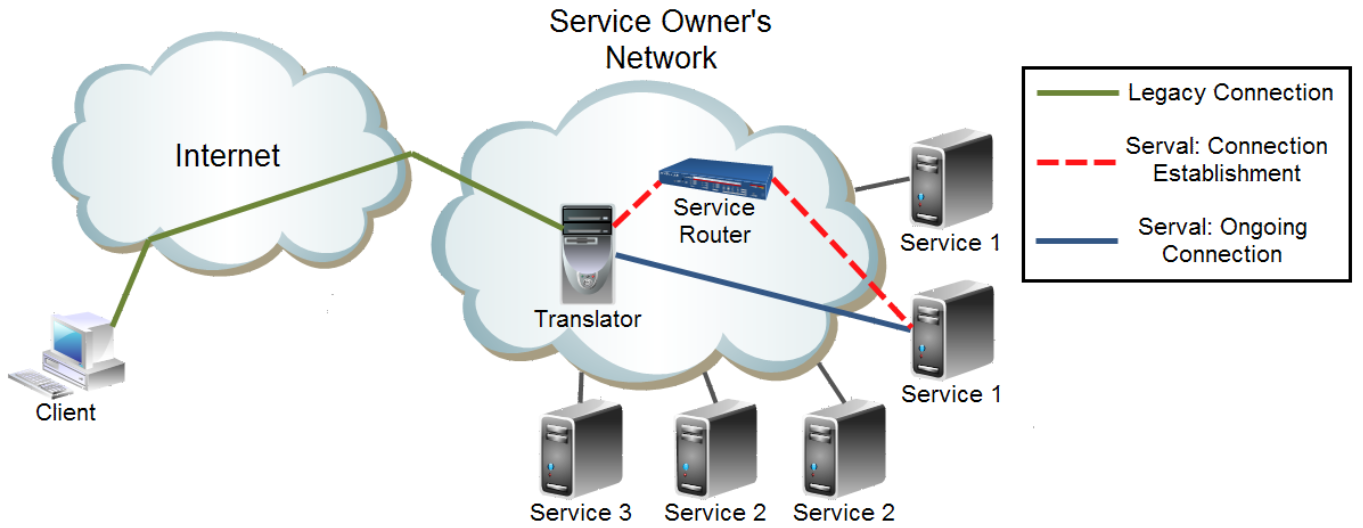
\includegraphics[scale=0.25]{figures/Serval_translator}
\caption[Serval translator]{A Serval translator as an intermediary\\for communicating with legacy clients \cite{Podmayersky2011}.}
\label{fig:serval_translator}
\end{figure}
The Internet has expanded in a level where migrating to a new architecture through a coordinated "flag day", where we disconnect all devices in order to cold-plug update them, is an unnegoatiable scenario.
Downtime, unreachable hosts running on embedded hardware, telecommunications, are only a few of the reasons that induce a gradual strategy when it comes to adopting Serval.
\\ \indent As observed in similar examples, the ones expected to make the first move are service providers.
Both for the reason that they are greatly benefited by this migration, as well for their pertinent awareness.
In order to face the challenge of serving both legacy and Serval-enabled clients, Brandon Podmayersky implements a \emph{Serval translator} \cite{Podmayersky2011}, an intermediary service which can be hosted in a middlebox machine or on the server itself, and which bridges the connection between a service using Serval active sockets and legacy TCP/IP clients.
\\ \indent Serval translator works on the simple principle of exposing legacy TCP/IP interfaces to the outer network --may it be the Internet--, which are then translated to Serval active sockets.
The procedure is illustrated in Figure~\ref{fig:serval_translator}.
Legacy clients resolving a service name via a search mechanism, may it be DNS, get the public-facing IP address of the translator in front of the corresponding service.
Then they are connecting with that IP and a well-known port directly to the Serval translator, opening a typical AF\_INET socket.
The predefined port as anyone would expect can be the default legacy port of the service the client wants to reach (for a web server that would be port 80).
Note that a translator might be the first point of contact for multiple services, with its IP address registered --similar to a DNS A record-- for various service names and mapping requests to different ports to different services or service instances.
This mapping actually links an $<IP, port>$ tuple to a serviceID, which then can be resolved using the service table of SAL, or custom load balancing rules. 
After that, the translator takes care of the connection synchronization with the service, and splices\footnote{splice() is a system call introduced in the 2.6.17 kernel, that can move data between two file descriptors without copying between kernel address space and user address space\\ \url{http://linux.die.net/man/2/splice}.}
When the connection is terminated, the translator closes the sockets at both ends.
\\ \indent Using the Serval translator a service provider can handle requests from both legacy and Serval-ready clients.
Requests that have a serviceID get routed directly to the service instance, overpassing the translator.
However, on an established legacy connection, every single packet is processed by the translator, modifying headers and flags appropriately.
This indeed adds an overhead and indicates a possible single point of failure, but benchmarks show its performance is good enough to be deployed in real networks and a cluster of such translators can be used in a hierarchical schema.
\newpage
\subsection{Profiling the Serval prototype implementation}
Among the admirable headliners of Serval is the working prototype version of the proposed architecture.
In more than 28000 lines of code\footnote{Serval is an Open Source project, hosted at a public repository\\ \url{https://github.com/princeton-sns/serval/}.} covering functionality of the Service Access Layer (both in userlevel operation and as a Linux kernel module), bindings for multiple programming languages, a translator, libraries and examples for writing Serval compatible applications, and with a reported throughput comparable to the unmodified TCP/IP stack, it is clearly showcased the feasibility of the solution.

In this section we are profiling the prototype in regard to the following parameters:
\begin{enumerate} \itemsep1pt \parskip0pt 
\parsep0pt
  \item CPU Instructions and Cycles
  \item System Call execution times
  \item Execution time needed for the completion of a numbered iteration of requests
  \item Number of packers per request, bytes on the wire
\end{enumerate}
Then we will be presenting the results juxtaposed to the measurements of the unchanged TCP/IP stack and the AF\_INET family.

\paragraph{} Output was obtained on a HP Prodesk 600 G1 --Intel(R) Core(TM) i5-4570 @ 3.20GHZ, 4GB RAM-- machine running Ubuntu 11.04 (Natty Narwahl) kernel version 2.6.38-16-generic (rebuilt with debug symbols).

The profiling tools we used include gprof, perf, oprofile, valgrind, strace, zoom and google performance tools.
For the tests with gprof, valgrind, oprofile and strace, Serval module and http\_client were built with debug symbols.
Extra, for gprof testing, Serval was built with CFLAGS, LDFLAGS and CPPFLAGS equal to "-pg".

For the measurements we ported libmicrohttpd to use Serval active sockets.
Also, we implemented a simple HTTP client which supports both AF\_INET and the AF\_SERVAL socket families, depending on the options passed during the call.
For each case, we used the INET and Serval version of librehttpd and http\_client respectively.
Therefore, besides the connectivity parts, both INET and SERVAL versions are working with the same logic in creating, exchanging and processing requests.
This way we believe the tests can give unbiased results, which would not be the case if for example we used Apache server for INET and libmicrohttpd for SERVAL requests.

Source code of libmicrohttpd and http\_client, along with the integration of Serval patch in the build procedure of nginx, can be found in the Appendix (\ref{sec:appendix}).
Benchmark results are published in the ServalDHT repository \footnote{\url{https://github.com/misaakidis/ServalDHT}}.



\subsubsection{Serval's performance in the worst case scenario}
In a network architecture benchmarking what matters the most is its total throughput under a stress test.
In other words, the data rate of information (both headers and payload) and the number of packets that can be processed during a specific time frame.
An excellent tool for this case, \emph{iperf}, proved Serval's TCP throughput to be very close to the original TCP's one, almost fully utilizing a GigE interface. \nomenclature{GigE}{Gigabit Ethernet}
The authors explain that the existing small difference is due to missing optimizations in Serval's prototype.

We are examining Serval from a completely different perspective.
We dive into the implementation of SAL and serval.ko module and the overhead in using the Serval APIs.
And we do so in the worst possible scenario for an architecture that is establishing its own identifiers in the end host stacks.

It is SAL's responsibility to create the flows and synchronize the sockets in either side \footnote{Specifically for TCP, Serval is using the functionality that corresponds only to the ESTABLISHED state.}.
This means that when binding an active socket to a serviceID, the SAL must insert an entry into the flow table, register the service in the service table with a DEMUX rule and propagate the service registration to the network (may it be an anycast flood or a request to a singe service router).
Also, when connecting to a service, SAL must first convert a service name to a serviceID, resolve the serviceID, and finally establish a connection using CONTROL and SERVICE headers.
Correspondingly, closing a connection requires the exchange of packets with CONTROL headers.
In both cases, must-have checks like whether a serviceID is of an appropriate format, are more computational effort to the perquisite ones.

Once a connection has been established, the only significant overhead is the addition of a 12 bytes Serval header with the source and destination flowIDs, and the demultiplexing of incoming packets.
We can presume for those reasons, that Serval (and any other relative architecture) is struggling during the process of establishing a connection.

The case scenario we are testing is consisted of a client that connects to a service and requests information that can fit within a single response packet.
Since both the server and the client are running in the same machine, we can presume that the available bandwidth exempts network "links" from being responsible for a bottleneck.
The results show how well the Serval implementation can manage when it is pushed to the limit.



\newpage
\paragraph{Instructions and CPU Cycles} \hfill \\
Using perf performance counters subsystem in Linux \footnote{\url{https://perf.wiki.kernel.org/}}, we were able to benchmark the http\_client application with PF\_INET and PF\_SERVAL socket protocol families in a CPU cycle level.
There is definitely an increase in the Instructions and CPU cycles of the PF\_SERVAL version, as presented in Table \ref{table:cpu}, but taking a closer look in the perf output one will notice that there is a great increase in cache-misses and in the amount of branches.
Therefore the Instructions increase is a less biased index of the complexity added in the Serval port.
\begin{table}
\begin{center}
  \begin{tabular}{l||cc|cc|c}
  	\toprule
  	Metric			&	\multicolumn{2}{c}{PF\_INET}	&	\multicolumn{2}{c}{PF\_SERVAL}	&	Increase	\\
  	\midrule
    Instructions	&	690,559		&	$\pm$0.009\%	&	1,864,287	&	$\pm$0.054\%	&	169.9\%		\\
    CPU Cycles		&	1,019,096	&	$\pm$0.062\%	&	8,799,912	&	$\pm$0.191\%	&	763.5\%		\\
    Cache-misses	&	685			&	$\pm$1.417\%	&	72,893		&	$\pm$0.217\%	&	10541.3\%		\\
    Branches		&	125,548		&	$\pm$0.009\%	&	348,329		&	$\pm$0.057\%	&	177.4\%		\\
    \bottomrule
  \end{tabular}
  \caption[Benchmark: Instructions and CPU Cycles]{Instructions and CPU Cycles in 10000 runs of http\_client}
  \label{table:cpu}
\end{center}
\end{table}



\paragraph{System Calls execution times} \hfill \\
The results in Table \ref{table:stat} from stat user call \footnote{\url{http://man7.org/linux/man-pages/man1/stat.1.html}} show the independence of the time system calls need to complete, regardless the use of INET or SERVAL protocol family sockets.
This was expected and validated, since SAL in the kernel level is using the same system calls for its networking functions.
\textbf{\begin{table}
\begin{center}
  \begin{tabular}{l||c|c}
  	\toprule
  	Syscall			&	PF\_INET	&	PF\_SERVAL	\\
  	\midrule
    socket			&	0.145		&	0.070		\\
    setsockopt		&	0.160		&	0.118		\\
    connect			&	0.117		&	0.113		\\
    getsockname		&	0.300		&	0.552		\\
    send			&	0.089		&	0.086		\\
    recv			&	0.159		&	0.313		\\
    close			&	0.086		&	0.087		\\
    \bottomrule
  \end{tabular}
  \caption[Benchmark: System Call execution times]{Kernel System Calls execution times (in milliseconds)}
  \label{table:stat}
\end{center}
\end{table}}



\newpage
\paragraph{Finite Requests loop timing} \hfill \\
In this test we calculate --again using perf-- the milliseconds needed for the execution of a single request.
It is noteworthy that after a number of requests the execution time fails significantly.
Results listed in Table \ref{table:reqtime}
\begin{table}
\begin{center}
  \begin{tabular}{l||cc|cc|c}
  	\toprule
  	Requests	&	\multicolumn{2}{c}{PF\_INET}	&	\multicolumn{2}{c}{PF\_SERVAL}	&	Increase	\\
  	\midrule
    10			&	1.171		&	$\pm$2.171\%	&	1.845		&	$\pm$1.542\%	&	57.5\%		\\
    100			&	0.399		&	$\pm$7.248\%	&	0.686		&	$\pm$9.404\%	&	71.9\%		\\
    1000		&	0.590		&	$\pm$5.835\%	&	0.837		&	$\pm$7.751\%	&	41.9\%		\\
    \bottomrule
  \end{tabular}
  \caption[Benchmark: Requests execution times]{Requests execution times}
  \label{table:reqtime}
\end{center}
\end{table}



\paragraph{Packets specific metrics} \hfill \\
After all, we are focusing on the packets sent for each HTTP request.
Serval again has to send 5 more packets with control headers for the establishment and closing of the connection.
Finally there is an increase in the bytes transferred on the wire.
It is wise to highlight at this point that in a case where the payload would need to be split in more packets, or the conenction to be used as a stream for communication, that the observed overhead of extra packets would be negligible, and only the 12-byte header of serval would add bits on the stream.
\begin{table}
\begin{center}
  \begin{tabular}{l||c|c}
  	\toprule
  	Metric				&	PF\_INET	&	PF\_SERVAL	\\
  	\midrule
    Packets/request		&	10			&	15			\\
    Bytes/request		&	922			&	1392		\\
    \bottomrule
  \end{tabular}
  \caption[Benchmark: Packets and bytes exchanged per request]{Packets and bytes exchanged per request}
  \label{table:packets}
\end{center}
\end{table}



\newpage
\subsubsection{Benchmark results files}
As a reference, you can find the results of performance testing in the public repository, under the \emph{benchmarking} directory.
Specifically for INET and SERVAL you will find:
\begin{enumerate}
  \item \emph{gprof\_httpclient}: Results from gprof profiling tool. One can see the call graph of http\_client. Execution is completed fast enough to show zero accumulated time with the 0.01 seconds samples.
  \item \emph{kcachegrindgui\_httpclient}: Annotated source code with valgrind's kcachegrind tool.
  \item \emph{kcachegrind\_httpclient}: Graphic representation of the call tree along with the Instructions of each function.
  \item \emph{libmicrohttpd\_wireshark.pcap}: Wireshark capture of INET and SERVAL sockets with the libmicrohttpd server.
  \item \emph{nginx\_wireshark.pcap}: Wireshark capture of INET and SERVAL sockets with the nginx server.
  \item \emph{opannotate\_httpclient}: Percentage of time spent on each file called (including shared libraries). Vmlinux corresponds to kernel space processes.
  \item \emph{perf\_httpclient}: Performance counter stats 10,000 requests.
  \item \emph{perf\_serval\_mod}: Map details of the serval dynamically shared object (dso). DSOs are the "gateway" between the user and kernel space, and act as the contact point when an application running in the user space makes a system call.
  \nomenclature{DSO}{Dynamically Shared Object}
  \item \emph{statc\_httpclient}: List of system calls.
  \item \emph{stat\_httpclient}: Ordered system calls with their execution time.
\end{enumerate}



\newpage
\subsubsection{Closing remarks on benchmark results}
Results from performance testing might be alerting.
As closing remarks of the benchmarking section, we would like to shape our thoughts on the topic.

Serval is a great, well-thought service-centric network architecture.
Its simple, genuine abstractions, its clean separation of the control and the data plane, its resilience in migration, its familiar APIs, all add upon a networking model which provides apparent benefits to service providers and users as well.

However, services have some congenital characteristics that are not met on all networked applications.
Above all, services rely on resolute connections.
Once the path is established, a flow is expected to retain its reachability and serve as the channel for constant communication with the other side.
A channel which ordinarily serves as the middle for large files exchange.
Thereupon, SYN packets are only a small proportion of the network traffic of services.
A small overhead thus in the connection establishment is acceptable, especially if it can prevent a future reinitiation of the same process.

In contrast, there are applications which are working in a completely different way.
Programs that wake up one in a day to send a single packet to a remote server.
Real time systems that have to deliver a small part of information to many recipients.
Embedded machines that produce burst data and which do not require every single packet to be delivered.

Those scenarios are far from rare.
VoIP, \nomenclature{VoIP}{Voice over IP} media streaming, online games, even the DNS itself are illustrative examples.
For many years now we have been treating them in a special way; connectionless communication.
UDP over TCP has been serving well in those situations that we want to send fast, limited amount of data or when we do not care about if the packets get delivered.

We understand that the tests conducted do not represent a common use case.
They indicate though a possible shortcoming of Serval and demonstrate an expected performance in the worst scenarios as described above.

In the long run, Serval should not be considered a nostrum.
As every networking paradigm, it servers best where it was originally intentioned to do so.
SAL's symbiotic capability with the TCP/IP stack gives us the final choice to reason in which circumstances to use the Serval APIs and when to follow the well-trodden path.